\documentclass[aspectratio=169]{beamer}
\usepackage{hyperref}
% \usepackage[T1]{fontenc}

% other packages
% \usepackage{latexsym,xcolor,multicol,booktabs}
% \usepackage{amssymb,amsfonts,amsmath,amsthm,mathptmx}
% \usepackage{calligra}
\usepackage{listings}  % graphicx, pstricks
\usefonttheme[onlymath]{serif}
% algorithms
\usepackage{algorithm}
\usepackage{algorithmic}
\usepackage{amsmath}
% draw
\usepackage{tikz}
\usepackage{cases}

\renewcommand{\today}{\number\year -\ifnum\month<10 0\fi\number\month -\ifnum\day<10 0\fi\number\day}
\renewcommand{\alert}[1]{\textbf{\color{stuba}#1}}
\newcommand{\ui}[2]{#1 _{\mathrm{#2}}}
% upright sub-index with variable
\newcommand{\uis}[3]{#1 _{\mathrm{#2}, #3}}

% The text inside the square brackets [] in the commands specifies their respective short versions that will appear in the header or footer of each slide in a Beamer presentation.
\author[M. Wadinger ]{Marek Wadinger, Michal Kvasnica}
% Authors with institution
% \author[M. Wadinger]{Marek Wadinger\inst{1}, Michal Kvasnica\inst{1} }
\title[Real-Time Outlier Detection]{Real-Time Outlier Detection with Dynamic Process Limits}
\subtitle{Process Control 2023}
\institute[STU]
{
\inst{} 
Institute of Information Engineering, Automation, and Mathematics \\
\textit{marek.wadinger@stuba.sk}
}
\date{}
\usepackage{STU}


% defs
\def\cmd#1{\texttt{\color[RGB]{0, 0, 139}\footnotesize $\backslash$#1}}
\def\env#1{\texttt{\color[RGB]{0, 0, 139}\footnotesize #1}}


\lstset{
    language=[LaTeX]TeX,
    basicstyle=\ttfamily\footnotesize,
    keywordstyle=\bfseries\color[RGB]{0, 0, 139},
    stringstyle=\color[RGB]{50, 50, 50},
    numbers=left,
    numberstyle=\small\color{gray},
    rulesepcolor=\color{red!20!green!20!blue!20},
    frame=shadowbox,
}

\begin{document}

\setbeamertemplate{headline}{}
\setbeamertemplate{footline}{}

\begin{frame}
    \titlepage
    \begin{figure}[htpb]
        \begin{center}
            \raisebox{-0.5\height}{
\includegraphics[width=0.1\linewidth]{figures/logos/logo_black_blue_transparent.pdf}}
            \raisebox{-0.5\height}{
\includegraphics[width=0.5\linewidth]{figures/logos/STU-FCHPT-anfh.pdf}}
        \end{center}
    \end{figure}
\end{frame}

\setbeamertemplate{headline}[smoothbars theme]
\setbeamertemplate{footline}[footline body]

% \begin{frame}
%     \tableofcontents[sectionstyle=show,subsectionstyle=show/shaded/hide,subsubsectionstyle=show/shaded/hide]
% \end{frame}


\section{Motivation}

\begin{frame}{Simulation Results}
    \begin{figure}[htpb]
        \begin{center}
            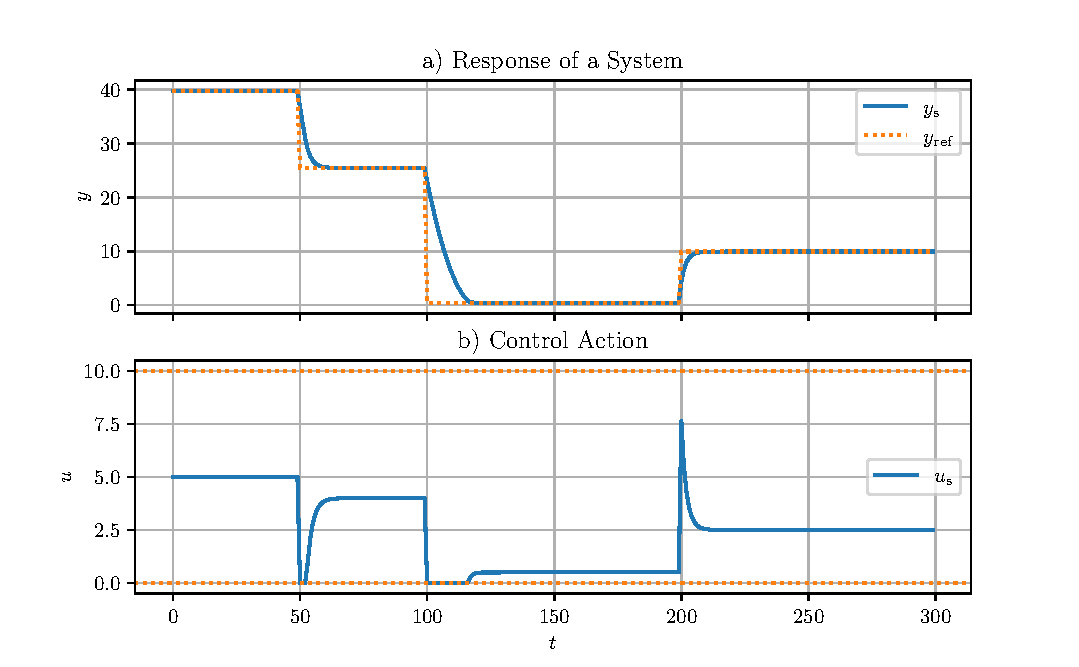
\includegraphics[width=0.75\linewidth]{../ilustrate/pc2023/simulation.pdf}
        \end{center}
    \end{figure}
\end{frame}

\begin{frame}{Practical Scenario}
    \begin{figure}[htpb]
        \begin{center}
            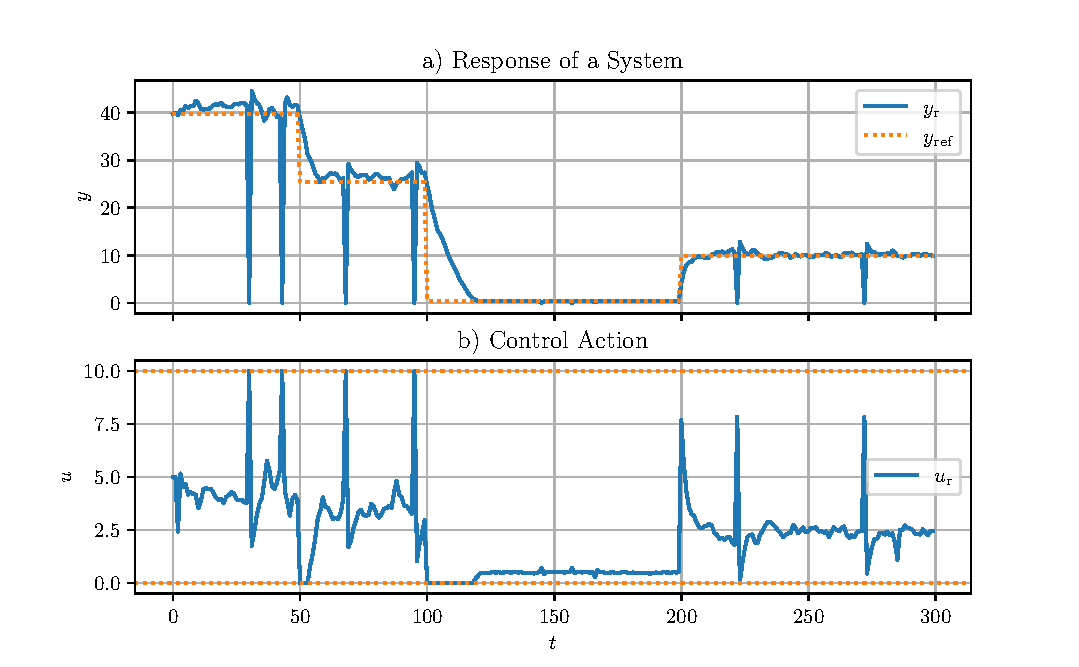
\includegraphics[width=0.75\linewidth]{../ilustrate/pc2023/real.pdf}
        \end{center}
    \end{figure}
\end{frame}

\begin{frame}{Control Engineering Meets Artificial Intelligence}
    \begin{figure}[htpb]
        \begin{center}
            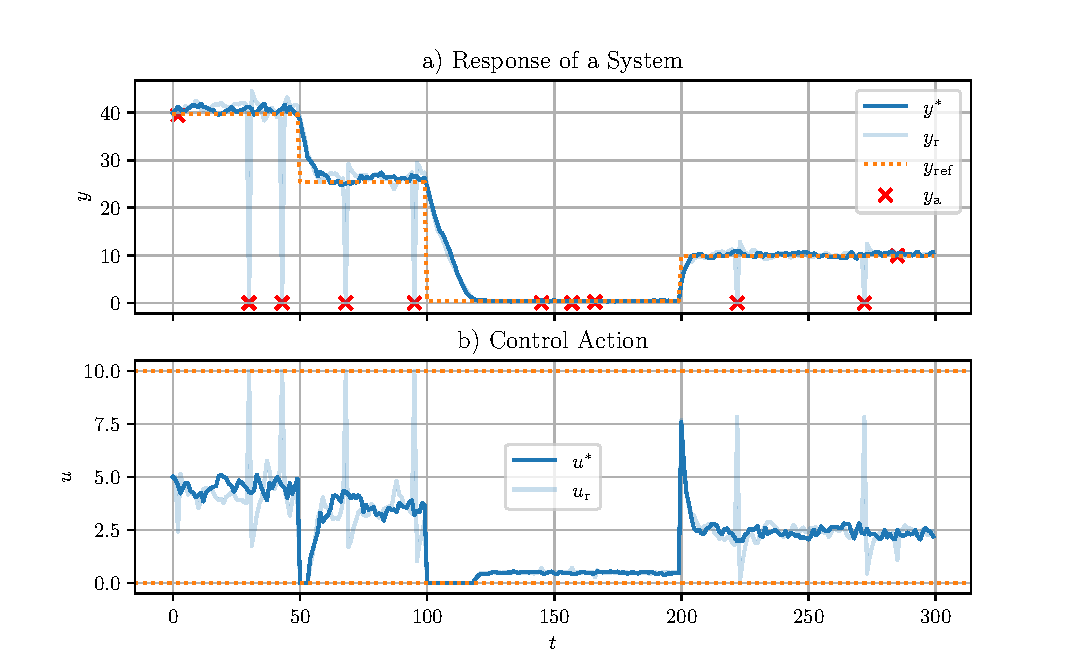
\includegraphics[width=0.75\linewidth]{../ilustrate/pc2023/imagined.pdf}
        \end{center}
    \end{figure}
\end{frame}


\section{Gaps in Existing Solutions}

\begin{frame}{Lack of Labels}
    \begin{figure}[htpb]
        \begin{center}
            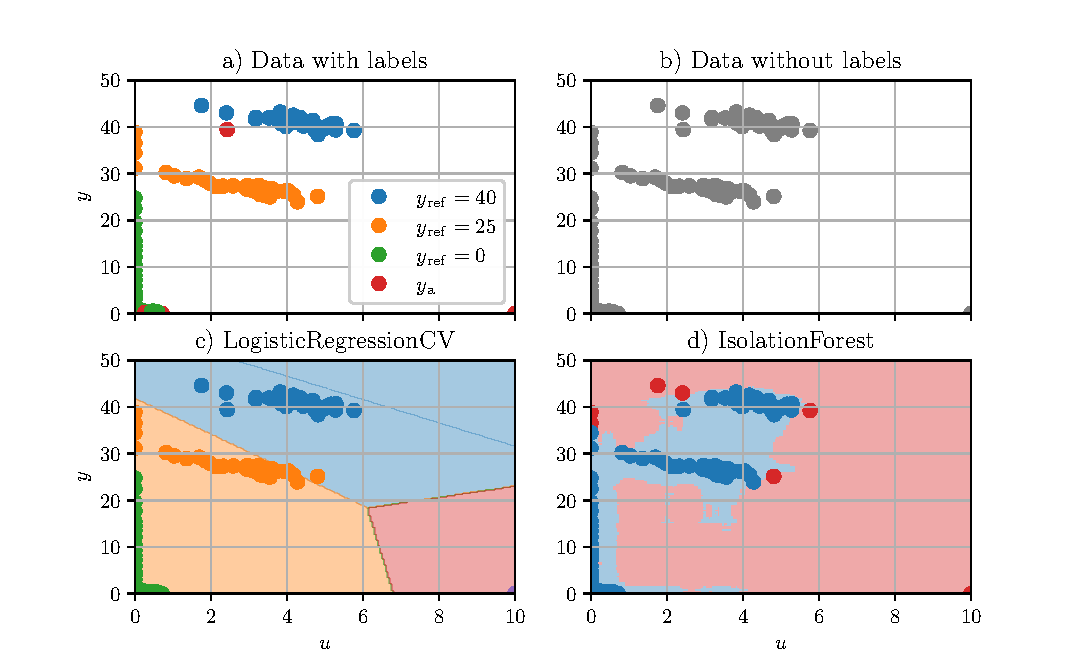
\includegraphics[width=0.75\linewidth]{../ilustrate/pc2023/un_supervised.pdf}
        \end{center}
    \end{figure}
\end{frame}

\begin{frame}{Changes in Distribution}
    \begin{figure}[htpb]
        \begin{center}
            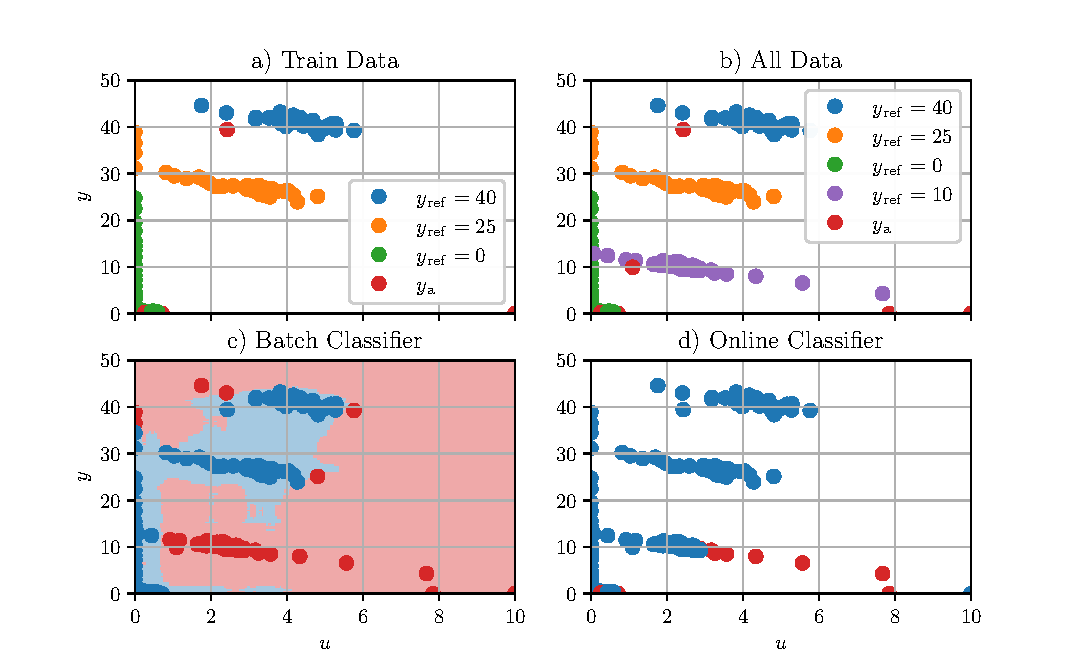
\includegraphics[width=0.75\linewidth]{../ilustrate/pc2023/online_freeze.pdf}
        \end{center}
    \end{figure}
\end{frame}

\begin{frame}{Goals}
    We need to make detector that:
    \begin{itemize}
        \item does not require huge amount of data
        \item adapts to unseen operation
        \item offers credible decision boundary
        \item does not alter operation of existing systems
        % \item Improves maintenance scheduling
    \end{itemize}
\end{frame}


\section{Proposed Approach}

\begin{frame}{Proposed Solution}
    Real-Time Outlier Detection with Dynamic Process Limits
    combining:
    \begin{itemize}
        \item online Learning
        \item outlier Detection
        \item self-supervised Learning
        \item soft Real-Time System
        \item invertible Probabilistic Model
    \end{itemize}
\end{frame}


\begin{frame}{Welford Algorithm}
    \begin{figure}
        \begin{center}
            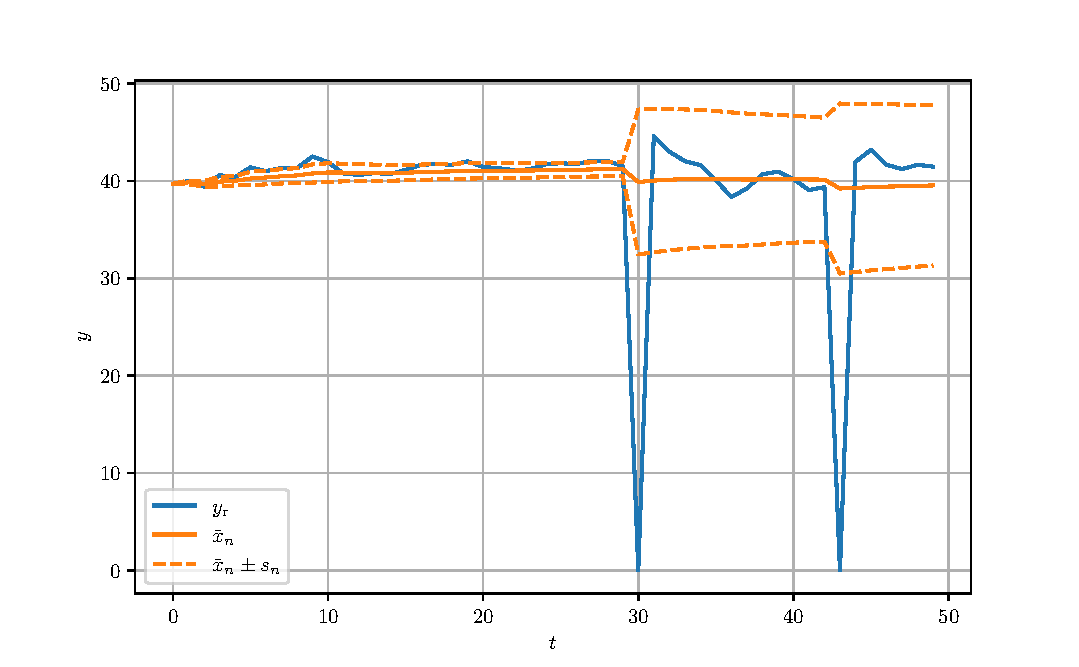
\includegraphics[width=0.62\linewidth]{../ilustrate/pc2023/welford.pdf}
        \end{center}
    \end{figure}
    \begin{table}
        \centering
        \begin{tabular}{c|c}
            {\color{green}{$+$}} One-Pass Algorithm & {\color{red}{$-$}} Adaptation Slows Down \\
        \end{tabular}
    \end{table}
\end{frame}

\begin{frame}{Inverse Welford Algorithm}
    \begin{figure}
        \begin{center}
            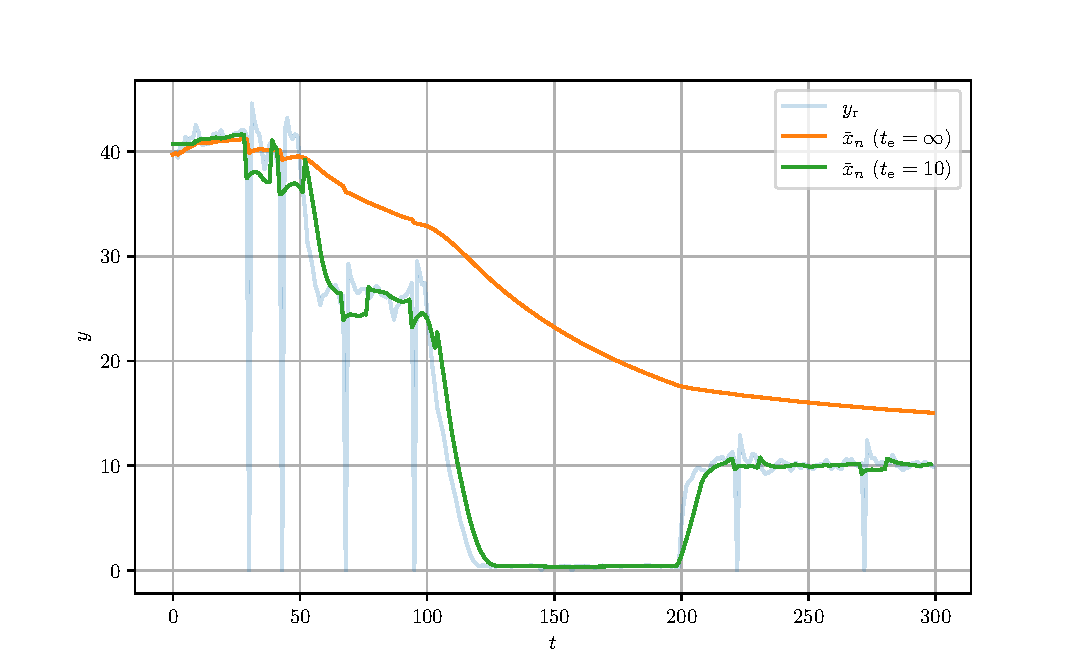
\includegraphics[width=0.62\linewidth]{../ilustrate/pc2023/welford_compare.pdf}
        \end{center}
    \end{figure}
    \begin{table}
        \centering
        \begin{tabular}{c|c}
            {\color{green}{$+$}} Constant Adaptation & {\color{red}{$-$}} Memorizes Data Window \\
        \end{tabular}
    \end{table}
\end{frame}

\begin{frame}{Distance-based Outlier Detection}
    \begin{figure}
        \begin{center}
            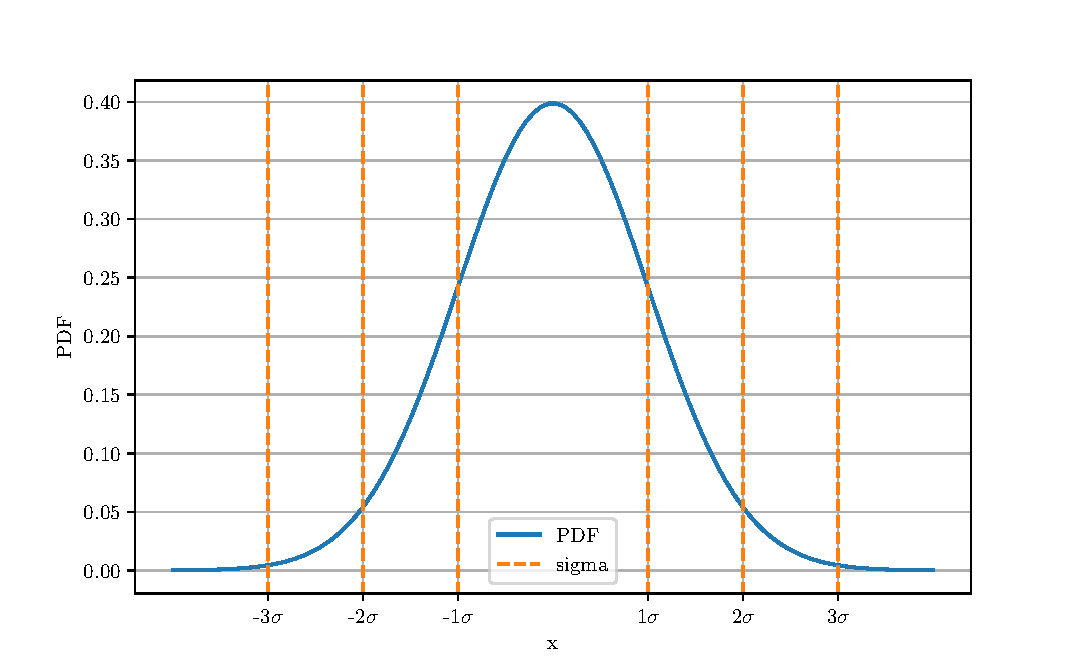
\includegraphics[width=0.62\linewidth]{../ilustrate/pc2023/sigmas.pdf}
        \end{center}
    \end{figure}
    \begin{subnumcases}{y_i =}
        0 & $\text{ if } q \leq F_{X}(x_i; \bar x_n, s_n)$ \nonumber\label{case:normal}
        \\
        1 & $\text{ if } q > F_{X}(x_i; \bar x_n, s_n)$ \nonumber\label{case:anomaly}
    \end{subnumcases}
\end{frame}

\begin{frame}{Self-Supervised Learning}
    \begin{figure}
        \begin{center}
            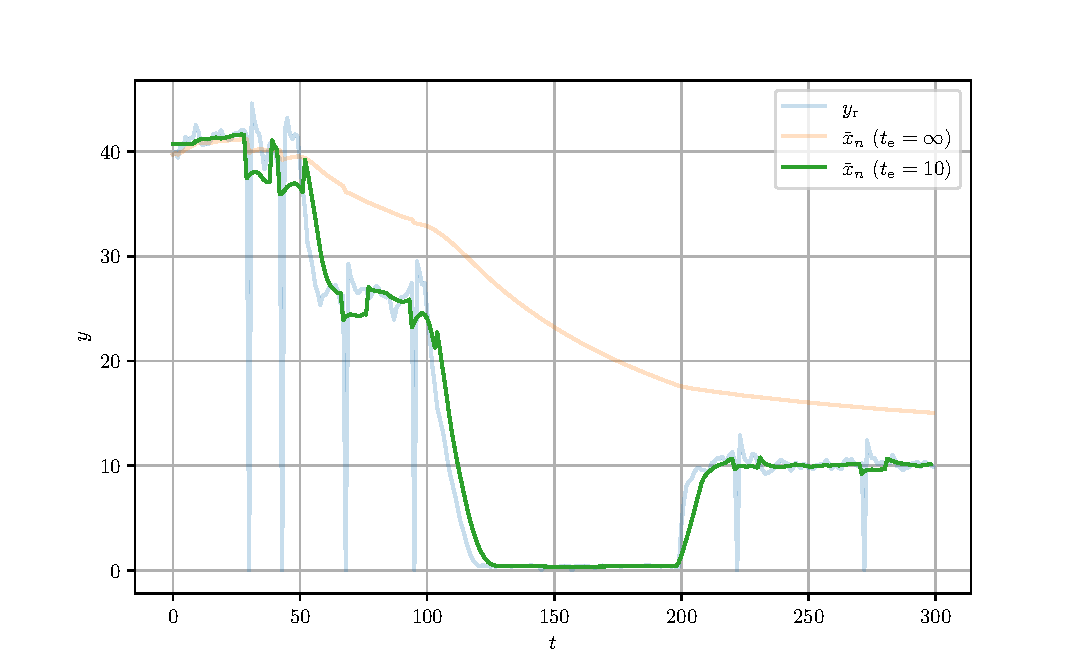
\includegraphics[width=0.62\linewidth]{../ilustrate/pc2023/welford_unstable.pdf}
        \end{center}
    \end{figure}
    \begin{subnumcases}{y_i =}
        0 & $\text{ if } q \leq F_{X}(x_i; \bar x_n, s_n)$ \nonumber  % \label{case:normal1}\tag{\ref{case:normal}}
        \\
        1 & $\text{ if } q > F_{X}(x_i; \bar x_n, s_n)$ \nonumber  % \label{case:anomaly1}\tag{\ref{case:anomaly}}
    \end{subnumcases}
\end{frame}

\begin{frame}{Self-Supervised Learning}
    \begin{figure}
        \begin{center}
            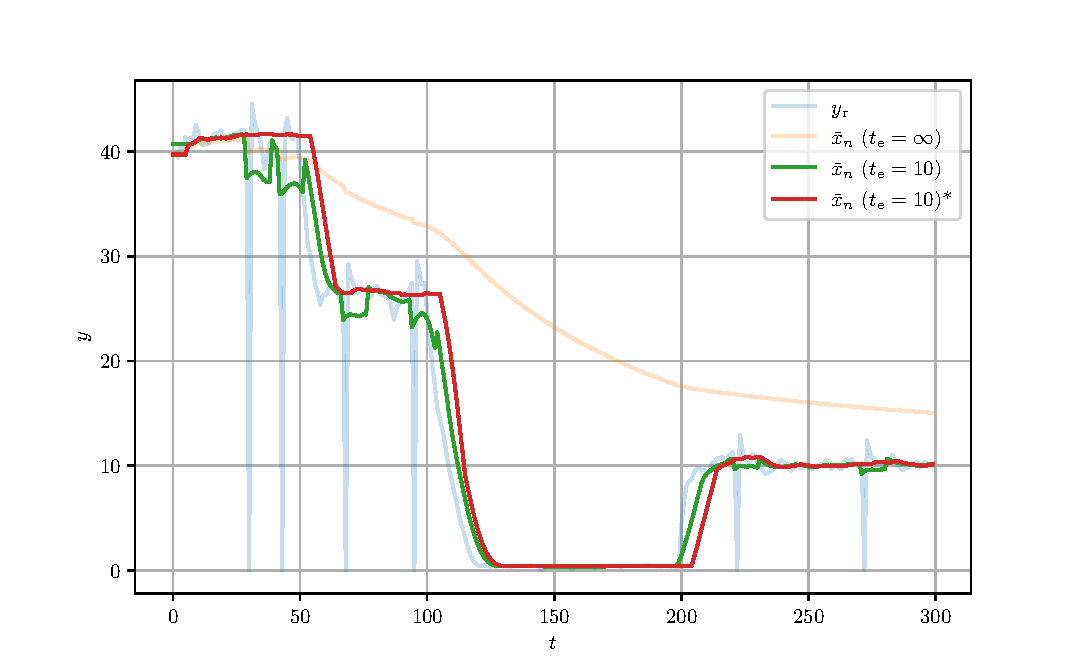
\includegraphics[width=0.62\linewidth]{../ilustrate/pc2023/welford_compare_prot.pdf}
        \end{center}
    \end{figure}
    \begin{equation}
        {\frac{\sum_{y\in Y}y}{|Y|}} > q\text{} \nonumber\label{eq:update}
    \end{equation}
\end{frame}

\begin{frame}{Inversion of CDF}
    \begin{figure}
        \begin{center}
            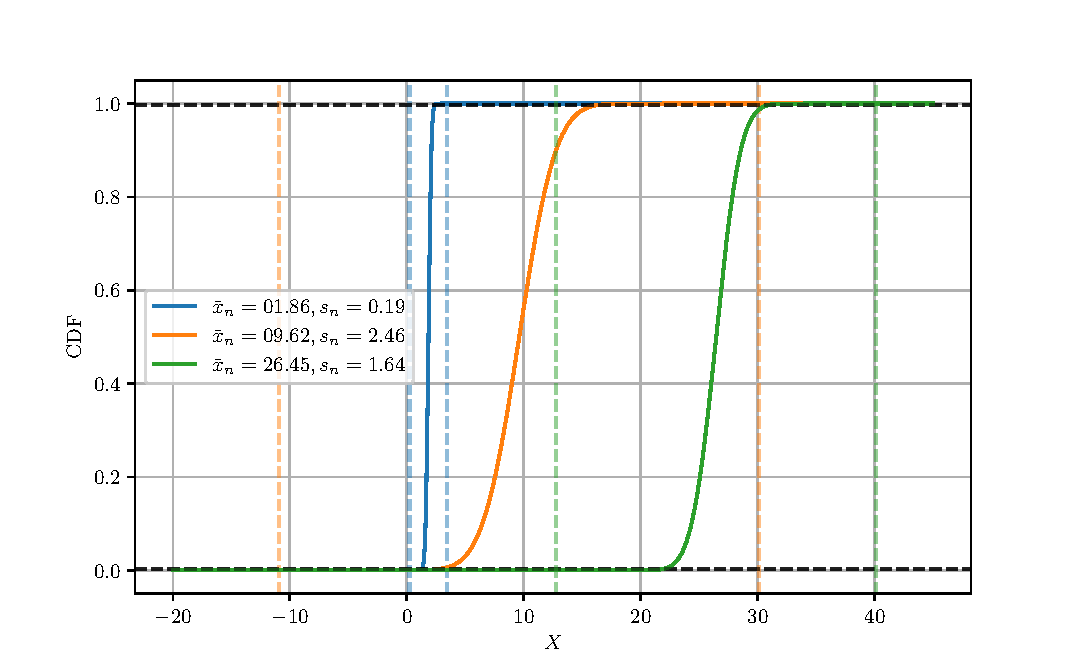
\includegraphics[width=0.62\linewidth]{../ilustrate/pc2023/cdf_ppf.pdf}
        \end{center}
    \end{figure}
    \begin{align*}
        \ui{x}{l} & = F_{X}(1 - q; \bar x_n, s_n)^{-1} \\
        \ui{x}{u} & = F_{X}(q; \bar x_n, s_n)^{-1}
    \end{align*}
\end{frame}

\section{Results}

\begin{frame}{ICDF-based Outlier Detection - BESS}
    \begin{figure}[htpb]
        \begin{center}
            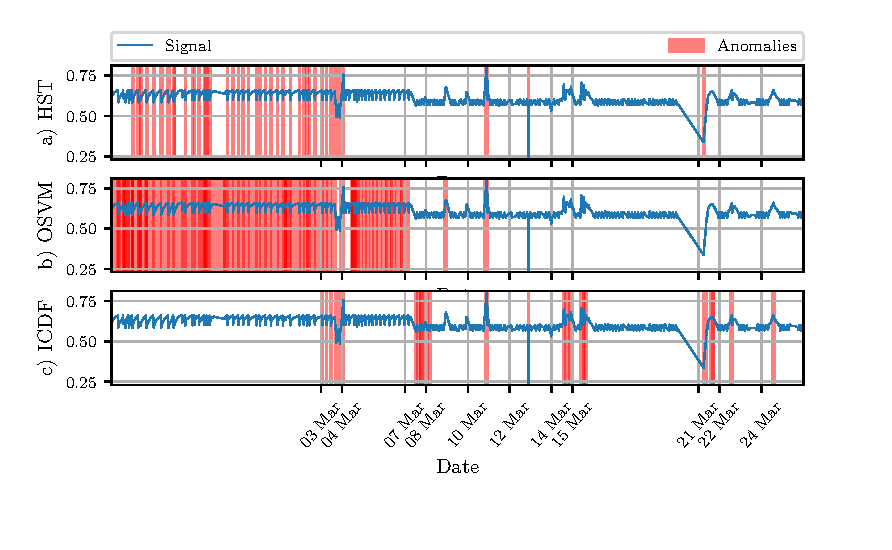
\includegraphics[width=0.78\linewidth]{figures/Average_Cell_Temperature_sliding_compare_anomalies.pdf}
        \end{center}
    \end{figure}
\end{frame}

\begin{frame}{ICDF-based Outlier Detection - Inverter}
    \begin{figure}[htpb]
        \begin{center}
            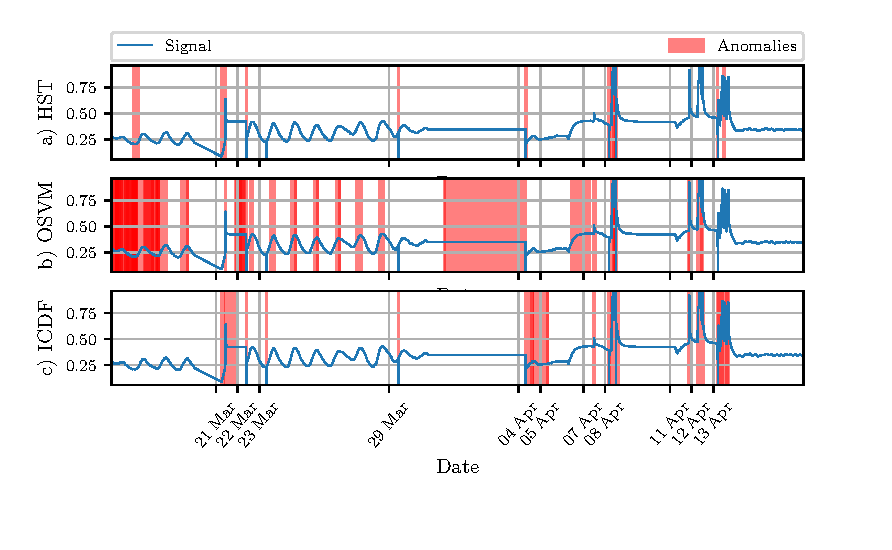
\includegraphics[width=0.78\linewidth]{figures/Inverter_Temperature_sliding_compare_anomalies.pdf}
        \end{center}
    \end{figure}
\end{frame}

\begin{frame}{Dynamic Process Limits}
    \begin{figure}[htpb]
        \begin{center}
            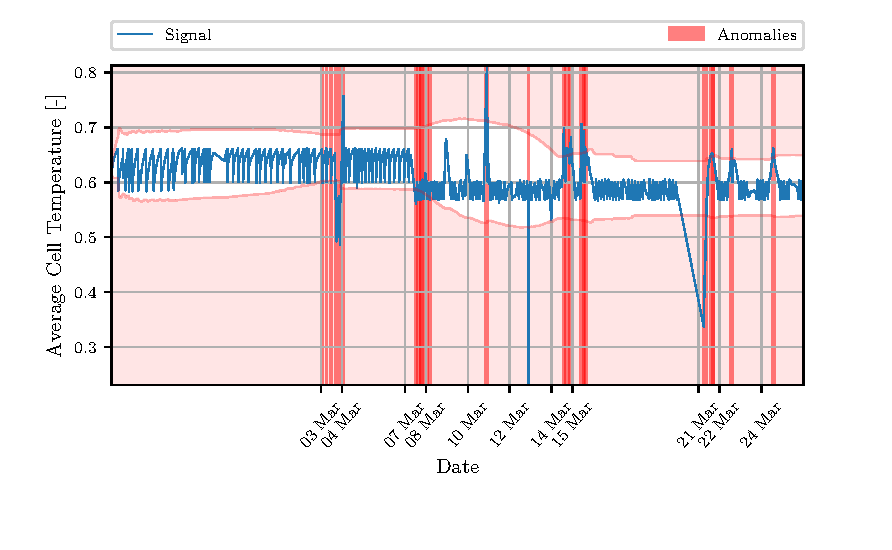
\includegraphics[width=0.78\linewidth]{figures/Average_Cell_Temperature_sliding_thresh_.pdf}
        \end{center}
    \end{figure}
\end{frame}

\begin{frame}{Dynamic Process Limits}
    \begin{figure}[htpb]
        \begin{center}
            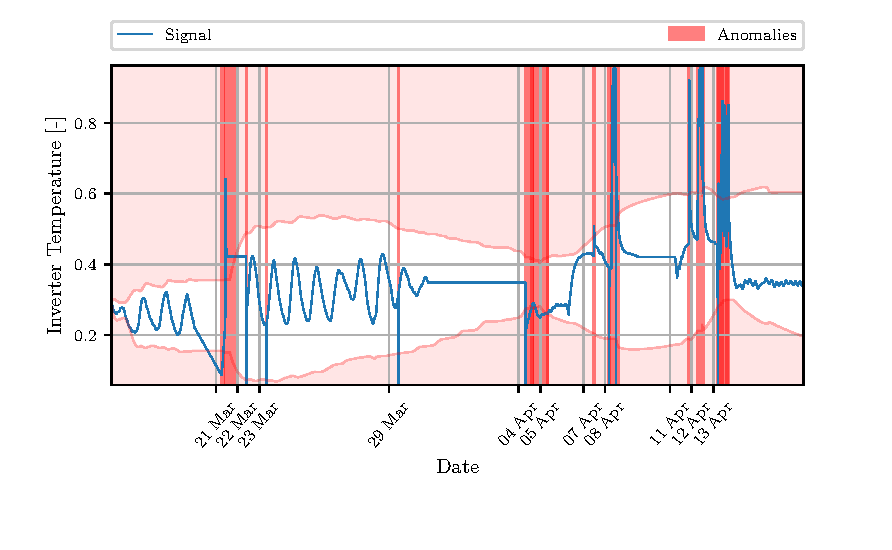
\includegraphics[width=0.78\linewidth]{figures/Inverter_Temperature_sliding_thresh.pdf}
        \end{center}
    \end{figure}
\end{frame}

\begin{frame}{Utilize Existing Infrastructure}
    \begin{figure}
        \centering
        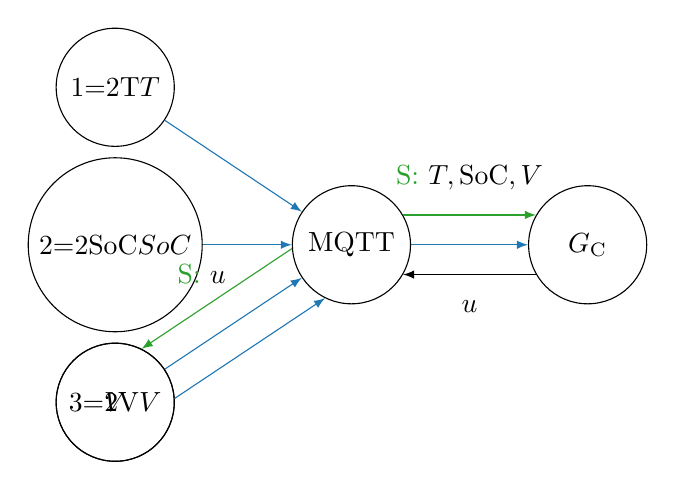
\begin{tikzpicture}
            % Draw big circle in the center
            \node[circle,draw, minimum size=1.5cm] (MQTT) at  (3, -2) {$\mathrm{MQTT}$};

            % Draw small circles on the left
            \def\labels{{"T", "SoC", "V"}}
            \xdefinecolor{subscribe}{RGB}{44, 160, 44}
            \xdefinecolor{signal}{RGB}{31, 119, 180}
            % Draw small circles on the left and add labels
            \foreach \y [count=\i] in {0, -2, -4} {
                    \def\label{\pgfmathparse{\labels[\i-1]}\pgfmathresult}
                    %\draw (0, \y) circle [radius=0.5cm] node {\label};
                    \node[circle,draw, minimum size=1.5cm] (\labels[\i-1]) at (0, \y) {\ifnumcomp{\i}{=}{2}{$\mathrm{\label}$}{$\label$}};
                    \ifnumless{\i}{3}
                    {\draw[-latex, signal] (\labels[\i-1]) -- (MQTT);}
                    {}
                }

            \node[circle,draw, minimum size=1.5cm] (V) at (0, -4) {$V$};
            % Connect middle circle to the circle on the right
            \node[circle,draw, minimum size=1.5cm] (G_C) at  (6, -2) {$\ui{G}{C}$};
            \draw[-latex, signal] (MQTT) -- (G_C);


            % Add subscribe lines
            \draw[-latex, subscribe] (MQTT) edge[bend right,draw=none] coordinate[at start](MQTT-b) coordinate[at end](G_C-b) (G_C)
            edge[bend left,draw=none] coordinate[at start](MQTT-t) coordinate[at end](G_C-t) (G_C)
            (MQTT-t) -- (G_C-t) node [pos=0.5,above=0.2cm] {S: {\color{black}{$T, \mathrm{SoC}, V$}}};
            \draw[-latex] (G_C-b) -- (MQTT-b) node [pos=0.5,below=0.2cm] {$u$};

            \draw[latex-, signal] (MQTT) edge[bend right,draw=none] coordinate[at start](MQTT-b) coordinate[at end](V-b) (V)
            edge[bend left,draw=none] coordinate[at start](MQTT-t) coordinate[at end](V-t) (V)
            (MQTT-t) -- (V-t);
            \draw[latex-, subscribe] (V-b) -- (MQTT-b) node [pos=0.4,above=0.2cm] {S: {\color{black}{$u$}}};

        \end{tikzpicture}
    \end{figure}
\end{frame}

\begin{frame}{Utilize Existing Infrastructure}
    \begin{figure}
        \centering
        \begin{tikzpicture}
            % Draw big circle in the center
            \node[circle,draw, minimum size=1.5cm] (MQTT) at  (3, -2) {$\mathrm{MQTT}$};
            % Draw small circles on the left
            \def\labels{{"T", "SoC", "V"}}
            \xdefinecolor{subscribe}{RGB}{44, 160, 44}
            \xdefinecolor{signal}{RGB}{31, 119, 180}

            % Draw small circles on the left and add labels
            \foreach \y [count=\i] in {0, -2, -4} {
                    \def\label{\pgfmathparse{\labels[\i-1]}\pgfmathresult}
                    %\draw (0, \y) circle [radius=0.5cm] node {\label};
                    \node[circle,draw, minimum size=1.5cm] (\labels[\i-1]) at (0, \y) {\ifnumcomp{\i}{=}{2}{$\mathrm{\label}$}{$\label$}};
                    \ifnumless{\i}{3}
                    {\draw[-latex, signal] (\labels[\i-1]) -- (MQTT);}
                    {}
                }
            % Connect middle circle to the circle on the right
            \node[circle,draw, minimum size=1.5cm] (G_C) at  (6, 0) {$\ui{G}{C}$};
            \draw[-latex, signal] (MQTT) -- (G_C);

            % Add subscribe lines
            \draw[-latex, subscribe] (MQTT) edge[bend right,draw=none] coordinate[at start](MQTT-b) coordinate[at end](G_C-b) (G_C)
            edge[bend left,draw=none] coordinate[at start](MQTT-t) coordinate[at end](G_C-t) (G_C)
            (MQTT-t) -- (G_C-t) node [pos=0.3,above=0.7cm] {S: {\color{black}{$T, \mathrm{SoC}, V, \color{red}{A}$}}};
            \draw[-latex] (G_C-b) -- (MQTT-b) node [pos=0.5,below=0.2cm] {$u^{\color{red}{*}}$};

            \draw[latex-, signal] (MQTT) edge[bend right,draw=none] coordinate[at start](MQTT-b) coordinate[at end](V-b) (V)
            edge[bend left,draw=none] coordinate[at start](MQTT-t) coordinate[at end](V-t) (V)
            (MQTT-t) -- (V-t);
            \draw[latex-, subscribe] (V-b) -- (MQTT-b) node [pos=0.4,above=0.1cm] {S: {\color{black}{$u^{\color{red}{*}}$}}};

            % Connect middle circle to the circle on the right
            \node[circle,draw, minimum size=1.5cm] (ICDF) at  (6, -4) {$\mathrm{iCDF}$};
            \draw[-latex, signal] (MQTT) -- (ICDF);

            % Add subscribe lines
            \draw[latex-, red] (MQTT) edge[bend right,draw=none] coordinate[at start](MQTT-b) coordinate[at end](ICDF-b) (ICDF)
            edge[bend left,draw=none] coordinate[at start](MQTT-t) coordinate[at end](ICDF-t) (ICDF)
            (MQTT-t) -- (ICDF-t) node [pos=0.5,above=0.2cm] {\color{red}{$A$}};
            \draw[latex-, subscribe] (ICDF-b) -- (MQTT-b) node [pos=0.7,below=0.7cm] {S: {\color{black}{$T, \mathrm{SoC}, V$}}};
            % Add text 

        \end{tikzpicture}
    \end{figure}
\end{frame}

\newcommand\blfootnote[1]{%
    \begingroup
    \renewcommand\thefootnote{}\footnote{#1}%
    \addtocounter{footnote}{-1}%
    \endgroup
    }

\begin{frame}{Summary}
    \begin{itemize}
        \item automated alerting without prior knowledge of process limits
        \item assessment of environmental conditions and device aging
        \item self-learning approach using streamed data
        \item sets dynamic threshold for individual signals
        \item seamless integration with existing IT infrastructure
    \end{itemize}
    % \let\thefootnote\relax\footnote{\tiny some text}
    
    \blfootnote{\tiny \textbf{Acknowledgements:} APVV-20-0261. VEGA 1/0490/23. Horizon Europe under the grant no. 101079342.}
\end{frame}

\begin{frame}{Follow-up research}
    \begin{figure}[htpb]
        \begin{center}
            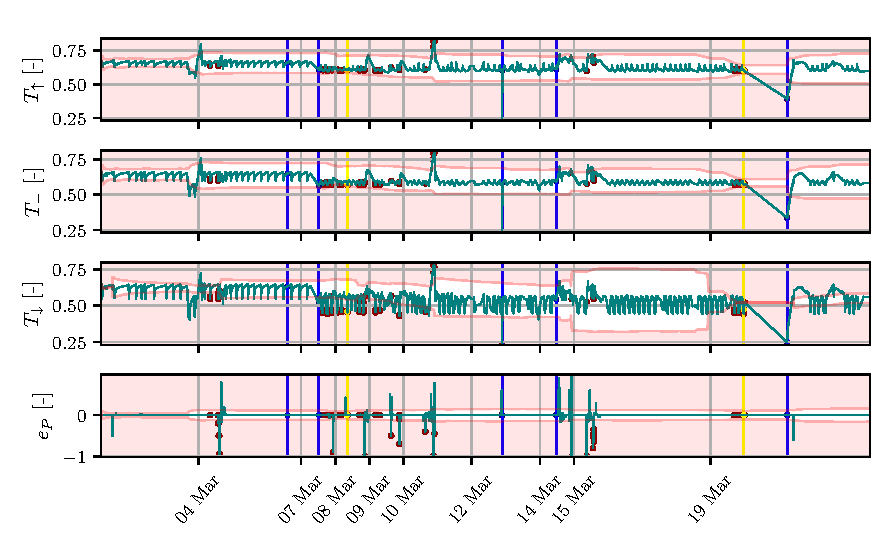
\includegraphics[width=0.65\linewidth]{../PC2023 Presentation/figures/cdc.pdf}
            \footnote{\tiny M. Wadinger and M. Kvasnica. Adaptable and interpretable framework for novelty detection in real-time iot systems. In Proceedings of the 62nd IEEE CDC, Singapore, 2023. under review.}
        \end{center}
    \end{figure}
\end{frame}

\begin{frame}{Online Anomaly Detection Workflow}
    \begin{algorithmic}[1]
        \scriptsize
        \algsetup{linenosize=\scriptsize}
        \renewcommand{\algorithmicrequire}{\textbf{Input:}}
        \renewcommand{\algorithmicensure}{\textbf{Output:}}
        \REQUIRE expiration period $\ui{t}{e}$, time constant $\ui{t}{c}$
        % sample mean $\bar x_0$, sample variance $s^2_0$, 
        \ENSURE  score $y_i$, threshold $\uis{x}{q}{i}$
        \\ \textit{Initialisation} :
        \STATE $i \leftarrow 1;~ n \leftarrow 1;~ q \leftarrow 0.9973;~ \bar x  \leftarrow x_0;~  s^2 \leftarrow 1$;
        \STATE compute $F_X(x_0)$ ;
        \\ \textit{LOOP Process}
        \LOOP
        \STATE {$x_i \leftarrow$ RECEIVE()};
        \STATE $y_i \leftarrow$ PREDICT($x_i$) ;
        \STATE $\uis{x}{q}{i} \leftarrow$ GET($q, \bar x, s^2$);
        \IF {\eqref{case:normal} \OR \eqref{eq:update}}
        \STATE {$\bar x$, $s^2 \leftarrow$ UPDATE($x_i, \bar x, s^2, n$)};
        \STATE $n \leftarrow n + 1$;
        \FOR {$x_{i-\ui{t}{e}}$}
        \STATE {$\bar x$, $s^2 \leftarrow$ REVERT($x_{i-\ui{t}{e}}, \bar x, s^2, n$)};
        \STATE $n \leftarrow n - 1$;
        \ENDFOR
        \ENDIF
        \STATE $i \leftarrow i + 1$;
        \ENDLOOP
    \end{algorithmic}
\end{frame}

\end{document}